This section shows the experimental and expected results of controlling a single joint via the Hubo-Ach system.
In this example the right shoulder pitch (RSP) is given a step input from 0.0 $rad$ to 0.4 $rad$.
The reference position $\theta_r$ is begin recorded as well as the actuator setpoint $\theta_c$ and the actual position of the joint $\theta_a$.
These definitions are also available in Table~\ref{table:recorded}

\begin{table}
\centering
\caption{States being recorded for the single joint step response test}
\begin{tabular}{l || c | c | c | c}
Signal      & Symbol     & Definition                    & Source      & Units \\
\hline
\hline
FeedForward & $\theta_r$ & Desired reference on the      & Hubo-Ach   & $rad$ \\
            &            & Hubo-Ach FeedForward Channel  &            &       \\
\hline
FeedForward & $\theta_c$ & Reference set to the actuator & Hubo-Ach   & $rad$ \\
\hline
Feedback    & $\theta_a$ & Actual position of joint as   & JMC        & $rad$ \\
            &            & measured from the encoders    &            &       \\
\hline
\end{tabular}
\label{table:recorded}
\end{table}



\begin{figure}[thpb]
  \centering
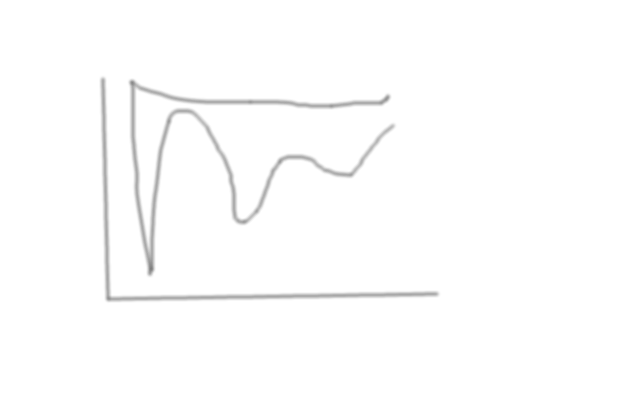
\includegraphics[width=0.8\columnwidth]{./pix/tmp.png}
  \caption{The commanded reference plotted against the actual reference recorded via Hubo-Ach and ground truth via CAN analyzing utilities.  In this plot the commanded reference is not automatically filtered by Hubo-Ach.  The commanded joint is the right shoulder pitch.}
  \label{fig:singleJointStep}
\end{figure}

Fig.~\ref{fig:singleJointStep} shows the results when a step input is applied and Hubo-Ach is in \textit{HUBO\_REF\_MODE\_REF\_FILTER} also know as passthrough mode.
This sets the what the desired reference on the \textbf{FeedForward} Hubo-Ach channel to the actuator's reference, i.e.:

\begin{equation}
 \theta_c = \theta_r
\end{equation}




\begin{figure}[thpb]
  \centering
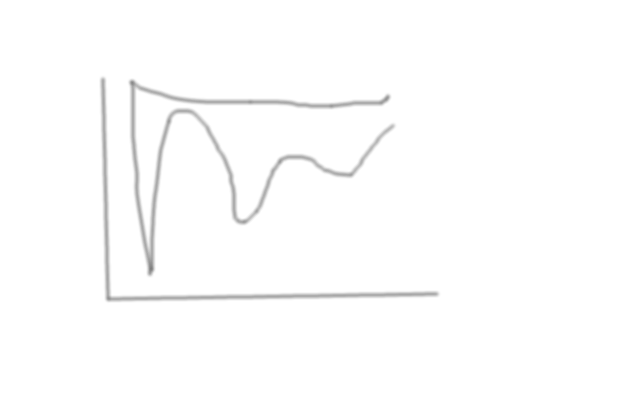
\includegraphics[width=0.8\columnwidth]{./pix/tmp.png}
  \caption{The commanded reference plotted against the actual reference recorded via Hubo-Ach and ground truth via CAN analyzing utilities.  In this plot the commanded reference is automatically filtered by Hubo-Ach.}
  \label{fig:singleJointStepFiltered}
\end{figure}